 

The telescope can only be controlled by a lead operator who has the correct credentials. To be a lead operator you will have credentials to control and monitor the telescope and these credentials are supplied by the Telescope Operations Manager. The telescope operates 24 hours a day, 7 days week and 365 days a year and there are 3 shifts a day split over 8 hours each. During the shift we have a lead operator who is responsible for controlling and monitoring the telescope system. Therefore there are three operators over a 24 hour period configuring and monitoring the telescope system at all times. Between the shifts one lead operator  hands over the system to the next operator. The paragraphs below describe in detail the procedure begging followed during the handover process.  
\section{Operator Handover Procedures}
Each Operator during the shift compiles a list or record  of the incidents that occured during  shift.  This record is called a handover document and this is different from the operations meeting minutes. The operator will update the incoming lead operator and also give this document to the next lead operator and this document will contain but not limited to this information below:
\begin{itemize}
\item{} What is currently being done with the telescope?
\item{} What observation is coming up after the current one?
\item{} What receptors are available and what receptors are expected back from maintenance?
\item{} What resources have been booked out for. maintenance and when - who to contact to get them back?
\item{} What problems are currently opened under which subsystems - supplement? this with reading open-ended user logs and the checklist [\textbf{Appendix A}]"
\item{} What are the problems experienced and what does the incoming operator need to look out for?
\end{itemize}
\section{Booking resource for maintenance}
The lead operator during the morning shift will be required to make resources (AP, Receivers, Digitiser, CBF etc) available to site technicians and engineers to conduct maintenance and upgrades. The resources will normally be booked for maintenance or upgrade at least a day before unless the resource is in error and cannot be used for operations. The lead operator will follow the process below:
\begin{itemize}
\item{} Check for booking in the Engineering Spreadsheet or Site calendar.
\item{} Mark the resource to maintenance - a log is automatically opened in the user logs. Add reason for booking in the log.
\item{} If the resource booked causes system downtime, add the ‘timeloss’ tag to the user log for system utilisation statistics reporting.
\item{} Alert maintenance staff or engineering staff after the resources have been made available. 
\item{} This information must also be added in the handover document. 
\end{itemize}
\section{ Receiving a resource after maintenance or an update}
\begin{itemize}
\item{} During the handover, check the control status of the resource \sensor{ap.control} sensor in sensor list  as shown in \textbf{Figure}~\ref{fig:image98}.

 \begin{itemize}
\item[$\circ$] If it is in remote - usable
\item[$\circ$] If it is in local/manual/e-stop - must be reset by technician
\end{itemize}

\begin{figure}[!thb]
	\centering
	%\includegraphicsdpi{100}{}{bur1.png}     
	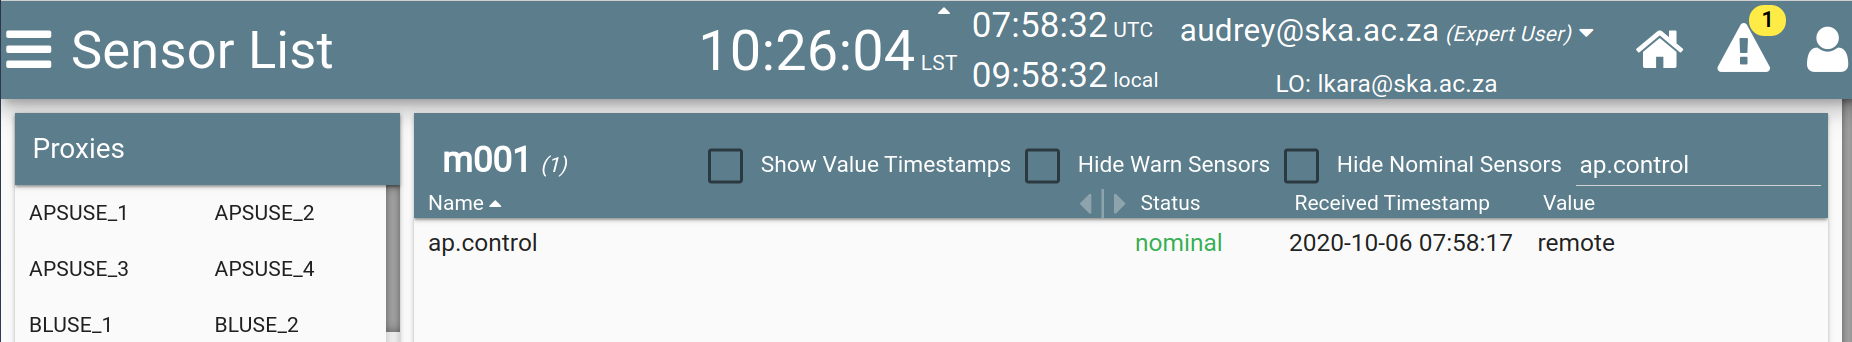
\includegraphics[scale=0.25]{Chapters/images/image98.png}
	
	%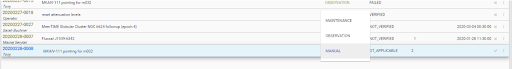
\includegraphics[resolution=100]{bur1.png}
	\caption{CAM GUI sensor list filtered with "Control"}
	\label{fig:image98}
\end{figure}
\item{} If in remote, check the health of the resource in detail

\begin{lstlisting}[style=DOS]
ssh kat@obs.mkat.karoo.kat.ac.za
./katsdpscripts/utility/check_ant.py --observer name --ant m0xx --proposal-id 22

\end{lstlisting}

Or 
\begin{lstlisting}[style=DOS]
./usersnfs/tiyani/meerkat_status.py --receiver rxl     

\end{lstlisting} (For L-band receivers)
\begin{lstlisting}[style=DOS]

./usersnfs/tiyani/meerkat_status.py --receiver rxu     

\end{lstlisting}
 (For UHF receivers)


\item{} Include the AP in the next observation to check signal quality
\item{} If a number of antennas are returning from maintenance and there is time before the next observation, create a small subarray with at least 4 antennas and run delay calibration, if there are less than 4 antennas available, build a subarray with those antennas but run three calibration script to check signal health.
\item{} Update OPS Catalyst page with correct number of APs available for use.

\section{Integrating a Receptor into Meerkat}
This must be done when an antenna has been in maintenance for an extended period of time or it was handed over to MPI for testing

Verify with the person who took the AP if they have changed anything in the digitiser,receiver or any other component configuration.
If there were changes made, talk to CAM to change what has been changed before testing the AP.
Run the \file{"check\_ant.py”} script as in the step above in 6.2
Mark the digitiser ready 
\begin{lstlisting}[style=DOS]
ssh kat@obs.mkat.karoo.kat.ac.za
ipython			
import katuilib
configure_cam("camcam","all")
cam.m0xx.sensor.dig`_selected_band.get_value()
cam.m0xx.req.digitiser_ready('l', timeout=60)
cam.m0xx.req.dig_select_band('l', timeout=60)
\end{lstlisting}




Where \component{m0xx} represents a receptor number e.g \component{m001}

\item{} Sync the digitiser using global sync - see next chapter.
\item{} Check the remaining hours left before the next global sync in sensor list of the CAM GUI as shown in \textbf{Figure}~\ref{fig:image68}.


\begin{figure}[!thb]
	\centering
	%\includegraphicsdpi{100}{}{bur1.png}     
	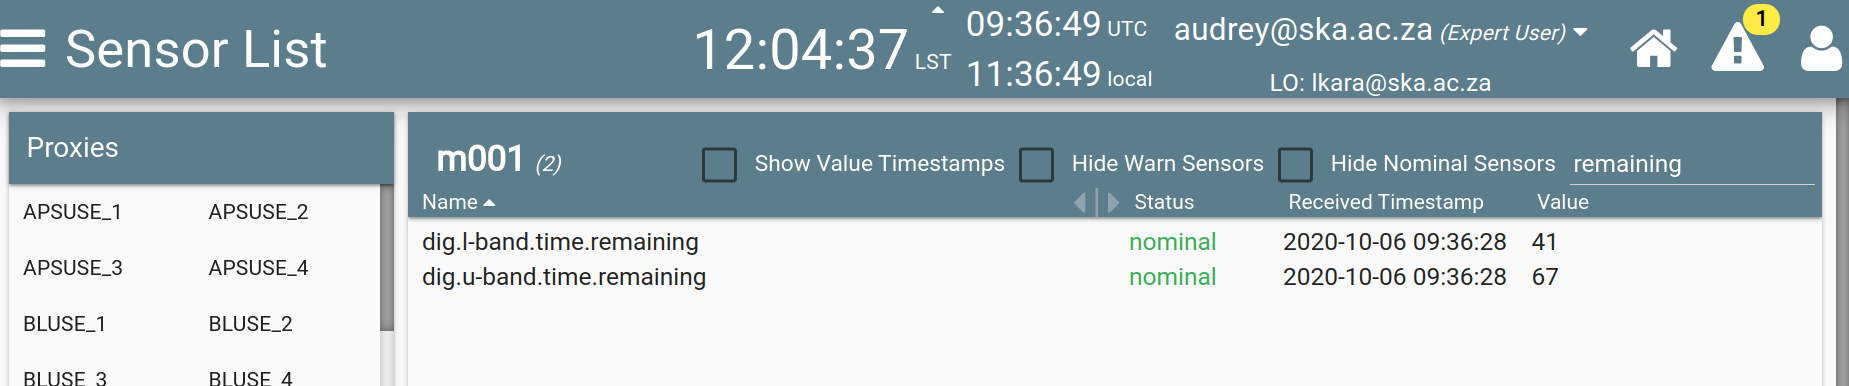
\includegraphics[scale=0.25]{Chapters/images/image68.png}
	
	%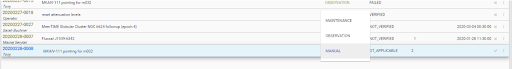
\includegraphics[resolution=100]{bur1.png}
	\caption{CAM GUI sensor list filtered by "remaining".}
	\label{fig:image68}
\end{figure}

These values above (41 \& 67) will indicate if global sync was successful or not for L and UHF$-$band digitisers.

\item{} Include the antenna in an array and run a calibrated delay script and see if it finds a solution. 
\begin{itemize}
\item [$\circ$] Look at the progress output of the delay cal script if the delay solutions are found.
		\item [$\circ$] During observation, look at the waterfall plot(signal displays) to see if there is a constant colour on its baseline. If the antenna looks noisy as in \textbf{Figure}~\ref{fig:image34} or has a rainbow, ask AoD to check its delay models.
\end{itemize}
 

\begin{figure}[!thb]
	\centering
	%\includegraphicsdpi{100}{}{bur1.png}     
	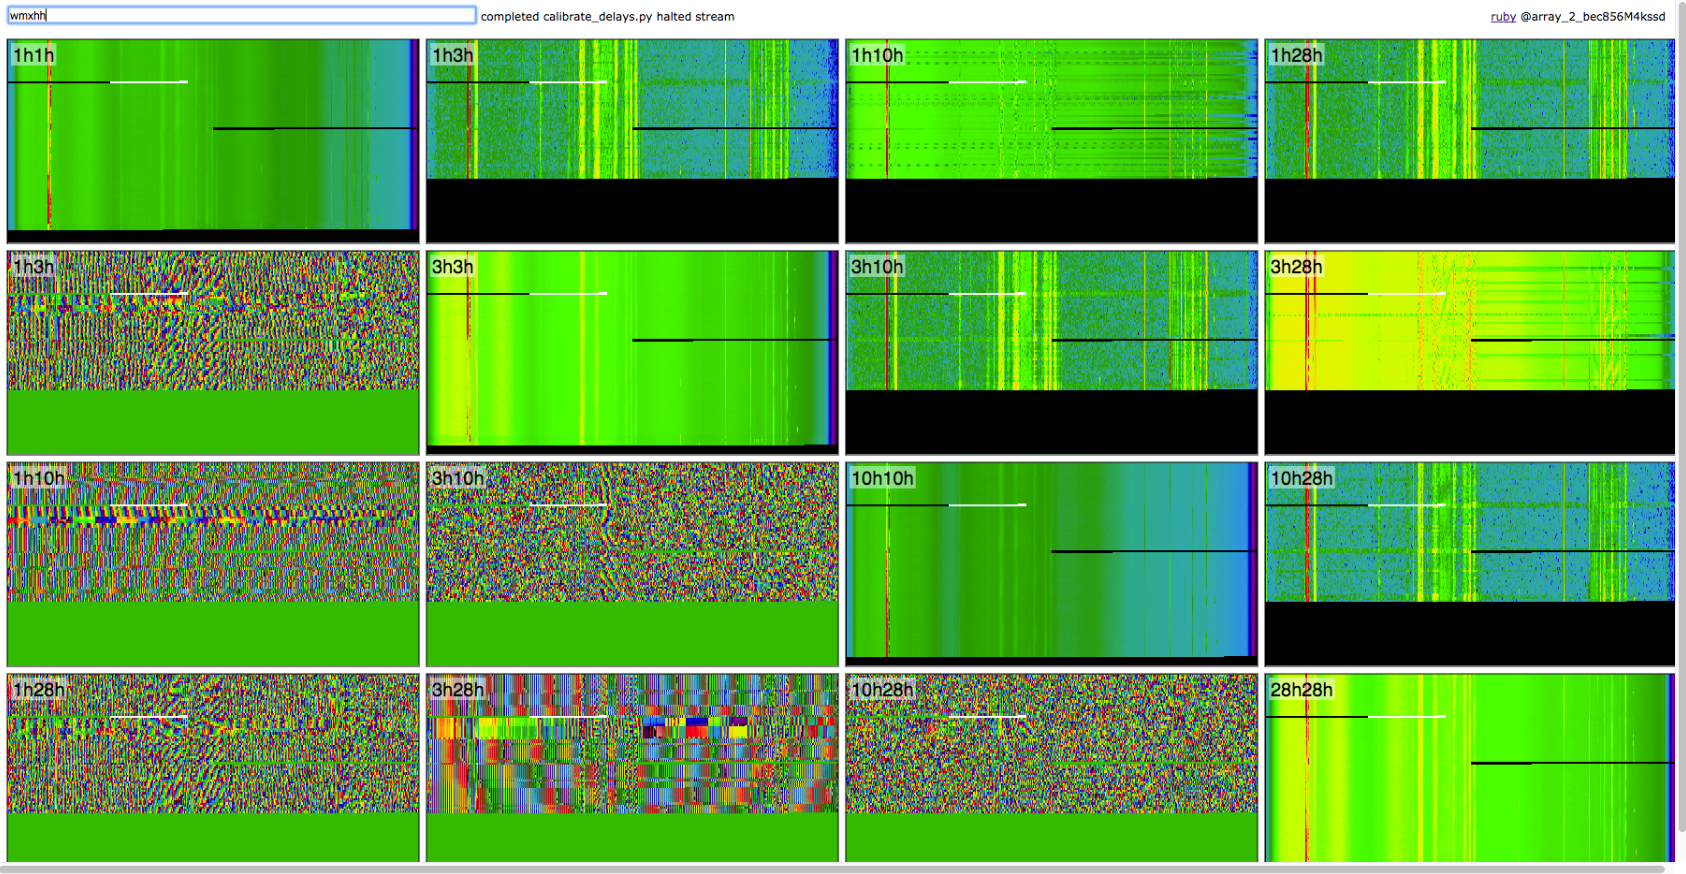
\includegraphics[scale=0.25]{Chapters/images/image34.png}
	
	%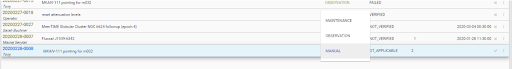
\includegraphics[resolution=100]{bur1.png}
	\caption{SDP waterfall plot.}
	\label{fig:image34}
\end{figure}

\item{} Before including the antenna in a Science observation communicate with the AoD about:
\begin{itemize}
	\item [$\circ$] interferometric pointing and notify operators to update pointing and delay models.
\end{itemize}

\item{} Update the Engineering Meerkat spreadsheet in the Owner tab.
\item{} Update the associated jira if necessary and close it.
\end{itemize}